\documentclass[a4paper,11pt]{article}
%\usepackage{jinstpub} % for details on the use of the package, please see the JINST-author-manual
\usepackage{lineno}
\usepackage{siunitx}
\usepackage{hyperref}
\linenumbers
\usepackage[backend=bibtex,style=ieee]{biblatex}
\addbibresource{biblio.bib}
\usepackage{url}
\usepackage{graphicx}
\usepackage{amsmath}
\usepackage{siunitx}
\usepackage[margin=1.1in]{geometry}
\usepackage{cleveref}

\graphicspath{{images/}}

% Proceedings/Special Issues
% Please note that this macro will be edited in production 
%% \proceeding{N$^{\text{th}}$ Workshop on X\\
%% When\\
%% Where}

%Gameplan
% get LED testing and VHDL code in, i might need uni access for these
%Write introduction and req with Sam
%keep on trucking with the points below


%THINGS TO DO FOR BEFORE PUBLICATION
%1. Write introduction and specifications
%2. go through each chapter and get the details right
%3. Insert figures
%4. Reread the whole thing multiple times
%5. Check formatting

%what sam said

%2 gothrough finish the thing
%use ~ between variables
%use unique reference names for each reference, labels
%


\setcounter{section}{-1}




\begin{document}
\title{\boldmath LED Light Injection System Technical Note}
\author{Balint Bogdan\footnote{bbogdan@liverpool.ac.uk}, Sam Jenkins}

\maketitle

\tableofcontents

\newpage

\section{Version history}
\begin{itemize}
\item v0.99 - First release by Balint circulated to Liverpool group for internal review
\item v1 - [Sam]: Ported over to github for continued development, as we hit compilation time on overleaf. Initial pass through to fix wording and rewrite some sections. Also integrating Warwick TN on OD diffuser
\end{itemize}

\newpage

\section{Introduction}
\label{sec:intro}

Hyper-Kamiokande is a large scale neutrino detector with 2 main sections, and inner (ID) and an outer detector (OD). The outer detector will have 122 injection points, each of them with a diffuser, which are illuminating a set of Photo Multiplier Tubes (PMTs) that are covered by a wavelength shifting plate, which has a response time of 10~ns. This means that the Light Injection System will have to be as precise as possible to make sure we can reduce the systematics of the Outer Detector (OD) by calibrating it accurately.

\section{Light Injection System Requirements}

For this system to be successful at calibrating the OD it must follow some rigid requirements. There will be 122 injection points, each of them must be illuminated by a single LED, so we must have 122 LEDs, and having several unused LEDs for quick changing in case an LED board stops working. There will be 5 lenght of fibre, 50~m, 80~m,106~m,124~m and 168~m. The light output after these fibres should be as uniform as possible, which is a challange, as different fibre length will have different dispersion, which will affect the pulse width, and attenuation, which will affect the light output. Pulse width should ideally be between 1-10~ns and the photon count from 1-15 million photons, but higher limits are preferable. The lower limits are not possible to achieve, as the fibre dispersion will create a minimum pulse width, which is 4.5~ns at 180~metres, and if we try to achieve large light output it will compromise our lower light output, so we can only achieve around 100,000 photons per pulse at minium. While these compromises are not ideal, the fibre selection limits our capabilities on hitting the required theoretical targets.
\section{Pulser Board}

\subsection{Pulser Board Overview}

The pulser board was designed to be a more efficient and compact version from the Super-Kamiokande UK Light Injection system, improving on efficiency, functionality, and light output. The pulser board, which may look complicated initially, is a rather simple board, designed for low cost production. In this technical note I will explain each circuit, component selection and design decisions. This is the version 0.9, which means it is almost the final version. V1.0 will be ready by September and will have only minor changes and adjustments compared to V0.9, mostly centered on removing the prototyping circuit and refinement. 


\subsection{Physical dimensions and construction}

The dimensions of the Printed Circuit Board (PCB) were selected to be as compact as practicable, while still providing sufficient area for the secure mounting of a fibre coupler and for the components. The final board size is 50~mm~$\times$~30~mm. This configuration permits electrically noisy component, such as switching power supplies and the Low Voltage Differential Signal to Transistor Transistor Logic (LVDS-to-TTL) converter to be positioned at a maximum distance from the switching circuitry, thereby minimising potential electromagnetic interference.
Although it is technically feasible to further reduce the board size, preliminary design studies and practical build indicated no substantial benefit in doing so. The board density cannot be significantly increased inside the crate due to Field Programmable Grid Array (FPGA) LVDS count and Eurocard dimension, and cost analyses revealed negligible differences associated with a smaller PCB footprint. Furthermore, the chosen dimensions provide an adequate area for the fibre coupler and the necessary mounting holes to affix the pulser board onto the Eurocard, thereby ensuring reliable optical alignment and mechanical stability.
The PCB is fabricated as a four-layer FR4  \cite{FR-4}  board with a thickness of 0.8~mm, in accordance with the standard construction offered by PCB Train/Newbury Electronics (these are trading names of the same manufacturer), see Figure~\ref{fig:PCBTrain0.84layer}. Refer to Figure~\ref{fig:PulserBoard0.93DTopandBottom} for the 3D model of the pulser board.\iffalse These are capitalised like this because these are the titles for the layers  \fi The Top Layer and Inner Top Layer are shown in Figure~\ref{fig:PulserBoard0.9TopLayers}, and the Inner Bottom Layer and Bottom Layer are likewise illustrated in Figure~\ref{fig:PulserBoard0.9BottomLayers}. A combined view of all PCB layers is provided in Figure~\ref{fig:PulserBoard0.9Overview}.


\begin{figure}[htbp]
\centering
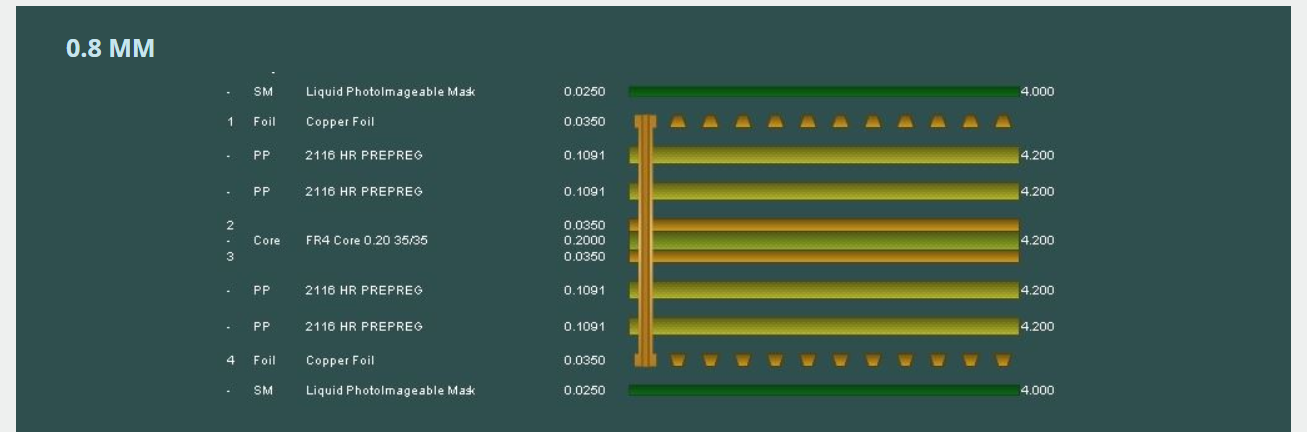
\includegraphics[scale=0.5]{PCBTrain0.84layer.png}
\caption{PCB Train's 4 Layer 0.8mm Layer Stack\label{fig:PCBTrain0.84layer}}
\end{figure}

\begin{figure}[htbp]
\centering
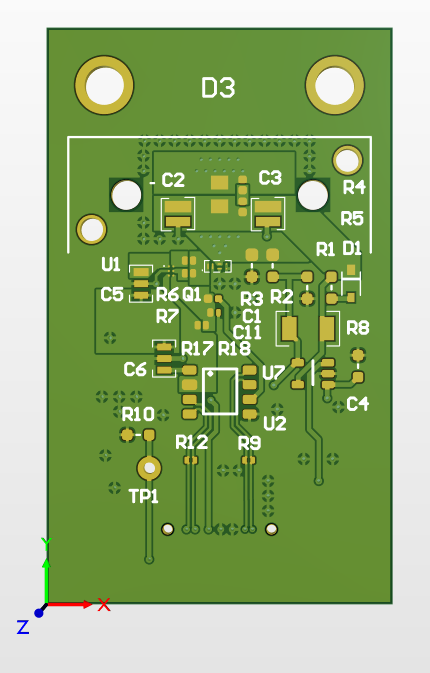
\includegraphics[scale=0.5]{PulserBoard0.93DTop.png}
\qquad
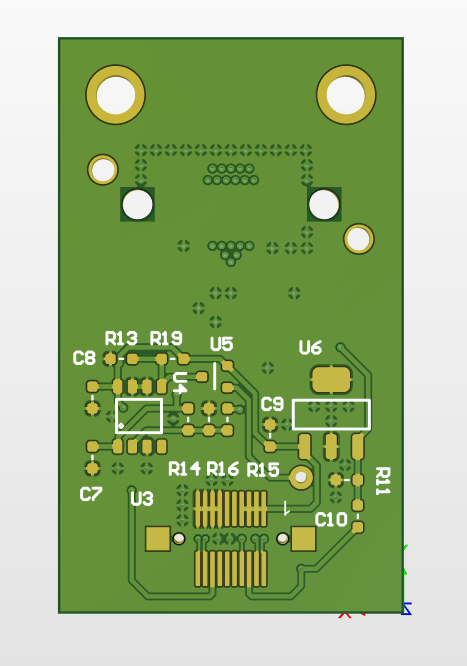
\includegraphics[scale=0.5]{PulserBoard0.93DBottom.png}
\caption{Pulser Board's 3D view Top and Bottom\label{fig:PulserBoard0.93DTopandBottom}}
\end{figure}

\begin{figure}[htbp]
\centering
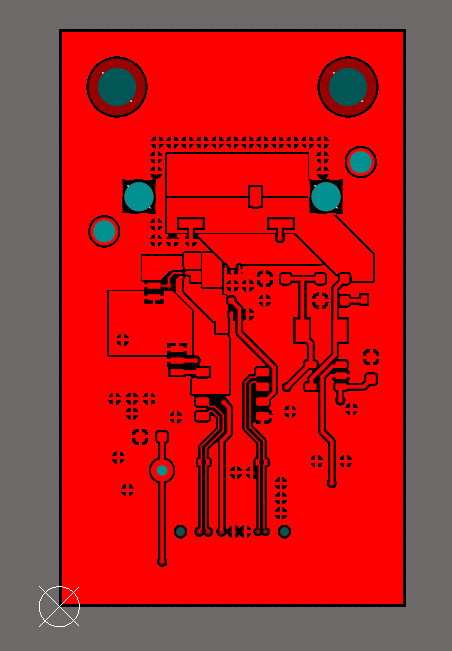
\includegraphics[scale=0.5]{PulserBoard0.9TopLayer.png}
\qquad
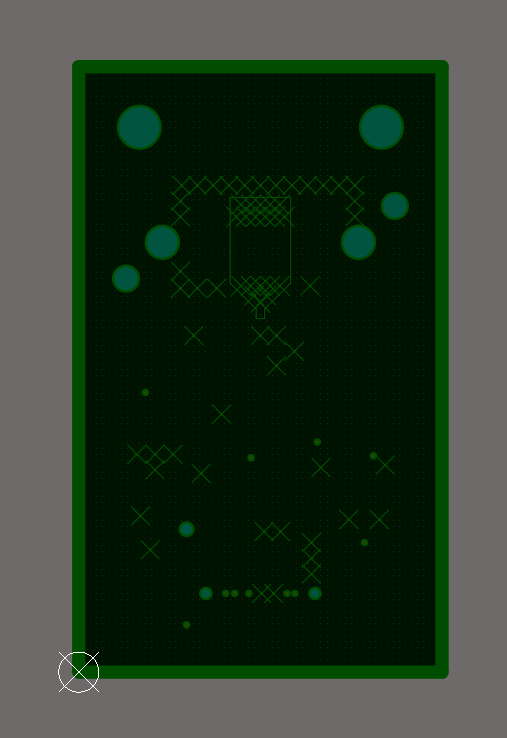
\includegraphics[scale=0.5]{PulserBoard0.9InnerTopGround.png}
\caption{Pulser Board Top and Inner Top Layer\label{fig:PulserBoard0.9TopLayers}}
\end{figure}

\begin{figure}[htbp]
\centering
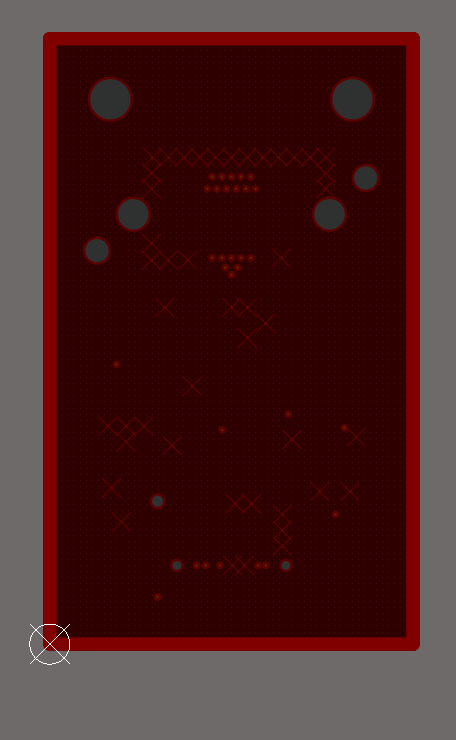
\includegraphics[scale=0.5]{PulserBoard0.9InnerBottomLayer.png}
\qquad
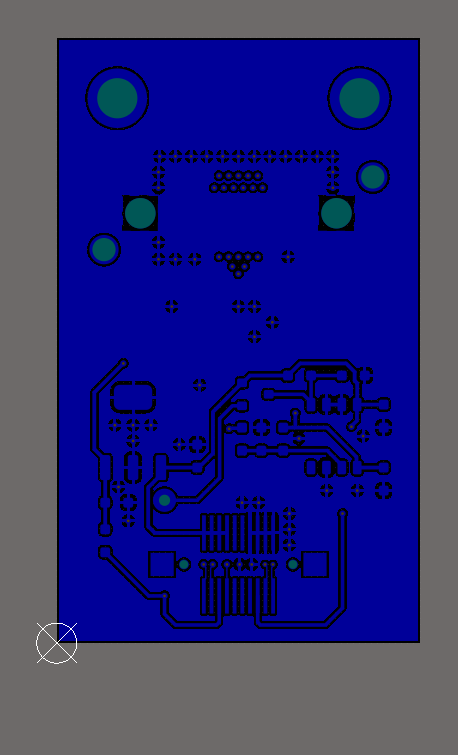
\includegraphics[scale=0.5]{PulserBoard0.9BottomLayer.png}
\caption{Pulser Board Inner Bottom and Bottom Layer\label{fig:PulserBoard0.9BottomLayers}}
\end{figure}


\begin{figure}[htbp]
\centering
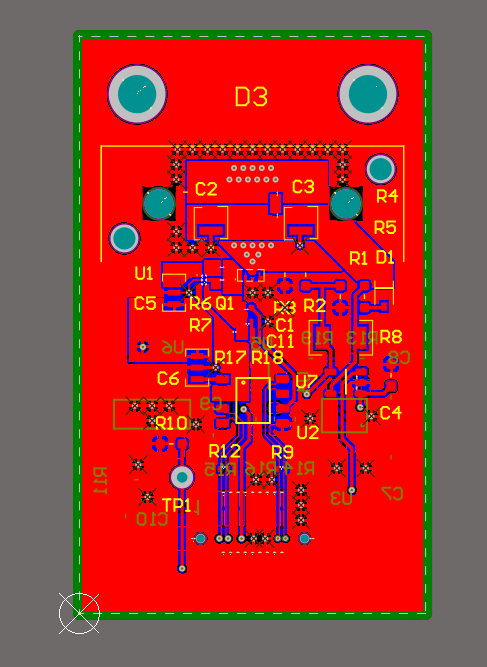
\includegraphics[scale=0.5]{PulserBoard0.9Overview.png}
\caption{Pulser Board Layer Overview\label{fig:PulserBoard0.9Overview}}
\end{figure}

\subsection{LED}

\subsubsection{Overview}

The LEDs are the most crucial component in the system because the electronics can be as perfect as possible,but the LEDs will output the light at the end. LEDs are usually not rated for such high-speed applications, which means we have to test and validate different LEDs ourselves, as there is no datasheet that can help us. The specification required were 1-10~ns clean single pulse, sub 400 nm wavelength, small surface mount package, narrow output beam so it can be coupled to a fibre with reduced losses and a good range of photon output. We have bought several LEDs, from Kingbright and LC-LED, and tested their performance.

%sort the part numbers out



\subsubsection{Switching Circuit}


The redesign process provided a valuable opportunity to evaluate a revised layout and new components for the switching circuit. 
Several enhancements have since been implemented in the revised switching circuit. Most importantly, the switching side of the layout has been rerouted. In contrast to the previous configuration, where current would flow through the limiting resistor regardless of the LED state, the updated design only allows current flow when the LED is active (refer to Figure~\ref{fig:Switching circuit}). This modification reduces both thermal dissipation and the overall power consumption of the system.
To modulate light intensity, a variable power supply is now employed to adjust the voltage supplied to the LED. This method has proven highly effective. Tests were conducted at various voltage levels using the full 181~m length of optical fibre—the maximum expected in deployment—and the resulting photon output ranged from approximately 100,000 to 20,000,000 photons per pulse. Refined testing results will be shown here shortly.
Further discussion regarding the implementation and performance of the variable voltage supply is provided in the power supply section. \iffalse insert reference \fi


\begin{figure}[htbp]
\centering
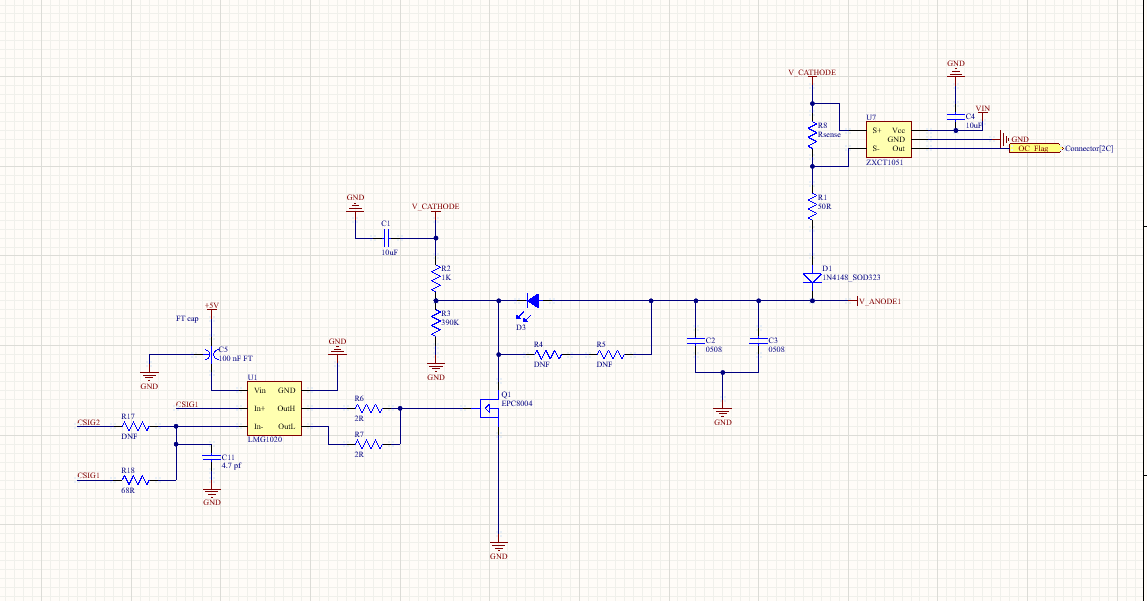
\includegraphics[scale=0.5]{Switching circuit.png}
\caption{Switching Circuit Layout with LMG1020 and over current IC, R4 is 6.8~nH inductor and R5 is 3R3 resistor\label{fig:Switching circuit}}
\end{figure}


\subsubsection{Switch Selection}

The previous iteration of the pulser board utilised a BFR92 \cite{BFR92} high-speed RF NPN switching transistor which was directly driven by a LVDS-to-TTL converter. In the redesign phase, alternative circuit topologies were explored—particularly those suitable for generating 1~ns and sub-nanosecond pulses. This investigation led to the adoption of gate driver circuits. Gate drivers are advantageous not only because they can power switches with challenging drive requirements, but also because sub-nanosecond electrical pulses can be achieved by modulating the enable pin with slight timing offsets. 
The fastest commercially available gate driver identified was the Texas Instruments LMG1020 \cite{LMG1020}. This device supports pulse widths down to 1,ns, with typical rise and fall times of 400~ps. Additionally, it features an enable pin that allows for precise nanosecond pulse shaping, refer to page 12 and 13 at the LMG1020 documentation. The LMG1020 is compatible with both Gallium Nitrite Field Effect Transistor (GaN)  and Metal Oxide Semiconductor Field Effect Transistor (MOSFET) switches, thereby broadening the scope for future component integration and experimentation. It is widely available and priced at £1.97 per unit in the quantities we will require for full production.
For the switching element, enhancement-mode GaN transistors manufactured by EPC were selected due to their superior switching characteristics. This recommendation originated from Nick Braam, an engineer at the University of Victoria, who contributed to the pulser board design for the mPMT system. Two EPC devices were shortlisted: the EPC2012 \cite{EPC2012} and EPC8004 \cite{EPC8004}. The EPC2012 offers a simpler footprint, which could reduce manufacturing defects; however, the EPC8004 features lower parasitic capacitance,see Figure~\ref{fig:EPC2012Cap} for the EPC2012 values and Figure~\ref{fig:EPC8004Cap} for EPC8004 values, leading to better high-speed performance.
To evaluate optical output performance, a 40~m length of FP400URT \cite{FP400URT} optical fibre, a Mouser-sourced 385~nm LED (ATS2012UV385 \cite{ATS2012UV385}), and a Hamamatsu H10721-210 \cite{H10721-210} photomultiplier tube were used. The EPC-based configurations exhibited nearly identical pulse shapes, whereas the BFR92-based circuit's pulse shape was less sharp at identical pulse widths~\ref{fig:BFR92PulseShape}. Consequently, the EPC8004~\ref{fig:EPC8004PulseShape} was chosen for implementation.
Optimal performance of the EPC GaN switches required careful layout considerations. A layout was developed in accordance with EPC's design guidelines \cite{EPCHSGuide}, targeting minimal parasitic inductance and capacitance. The design employs two layers placed directly above one another, utilising large copper planes and multiple vias to ensure uniform current distribution. The PCB will be fabricated and assembled by PCB Train, using their 0.8~mm thick, four-layer stack-up, which offers minimal inter-layer separation for optimal electrical performance (Figure~\ref{fig:PCBTrain0.84layer}). This same layout strategy was applied to the BFR92 circuit to provide a fair performance comparison.
A significant challenge at low pulse widths is the presence of a trailing edge or “tail” in the LED output. This effect arises due to charge accumulation and the intrinsic capacitance of the LED, resulting in extended decay times and pulse broadening (see Figure~\ref{fig:NoRLPulse}). To mitigate this, a parallel modified snubber circuit was implemented, consisting of a 6.8~nH inductor and a 3.3~$\Omega$ current-limiting resistor. Upon LED turn-off, the inductor generates an electromotive force (EMF) that actively extracts residual charge from the LED, accelerating its shutdown. The effectiveness of this approach is illustrated in Figure~\ref{fig:RLPulse}.
Additionally, two 0508 reverse-topology 100~nF capacitors have been incorporated. Their role is to act as local energy reservoirs, providing rapid current delivery to the LED during pulse operation, surpassing the response time of the main power supply.

\begin{figure}[htbp]
\centering
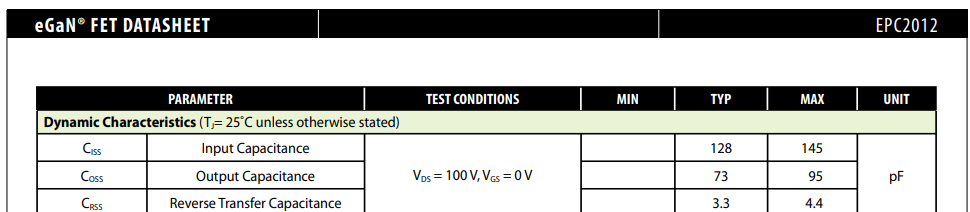
\includegraphics[scale=0.8]{EPC2012Cap.png}
\caption{EPC2012 Capacitance Values IC\label{fig:EPC2012Cap}}
\end{figure}

\begin{figure}[htbp]
\centering
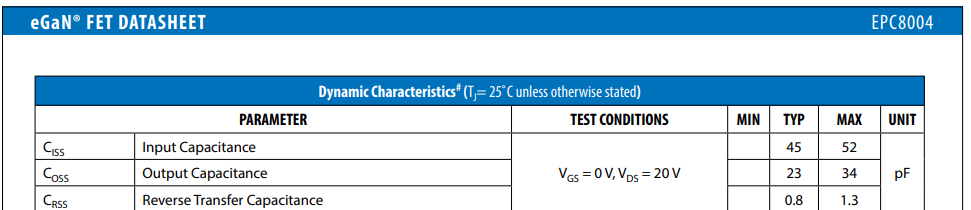
\includegraphics[scale=0.8]{EPC8004Cap.png}
\caption{EPC8004 Capacitance Values IC\label{fig:EPC8004Cap}}
\end{figure}

\begin{figure}[htbp]
\centering
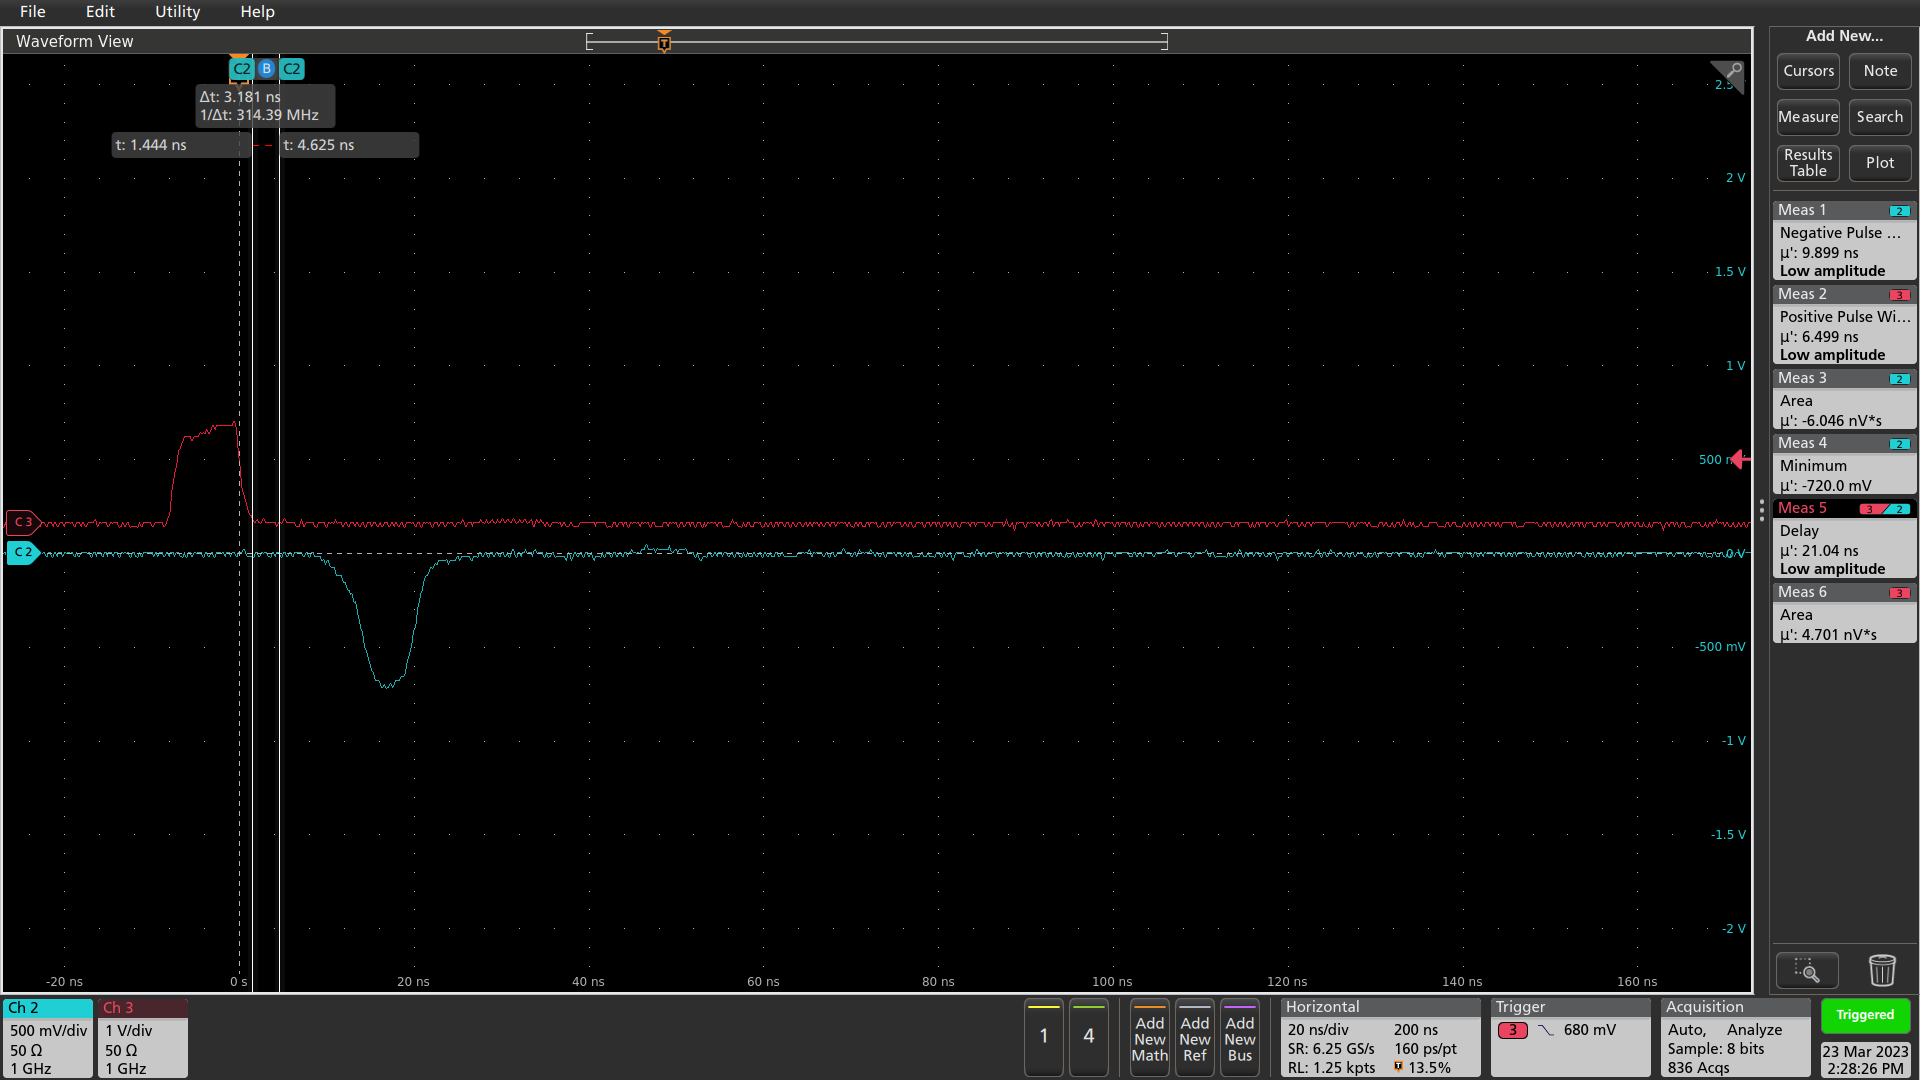
\includegraphics[scale=0.3]{bfr92st310nh_000.png}
\caption{BFR92 Pulse Shape\label{fig:BFR92PulseShape}}
\end{figure}

\begin{figure}[htbp]
\centering
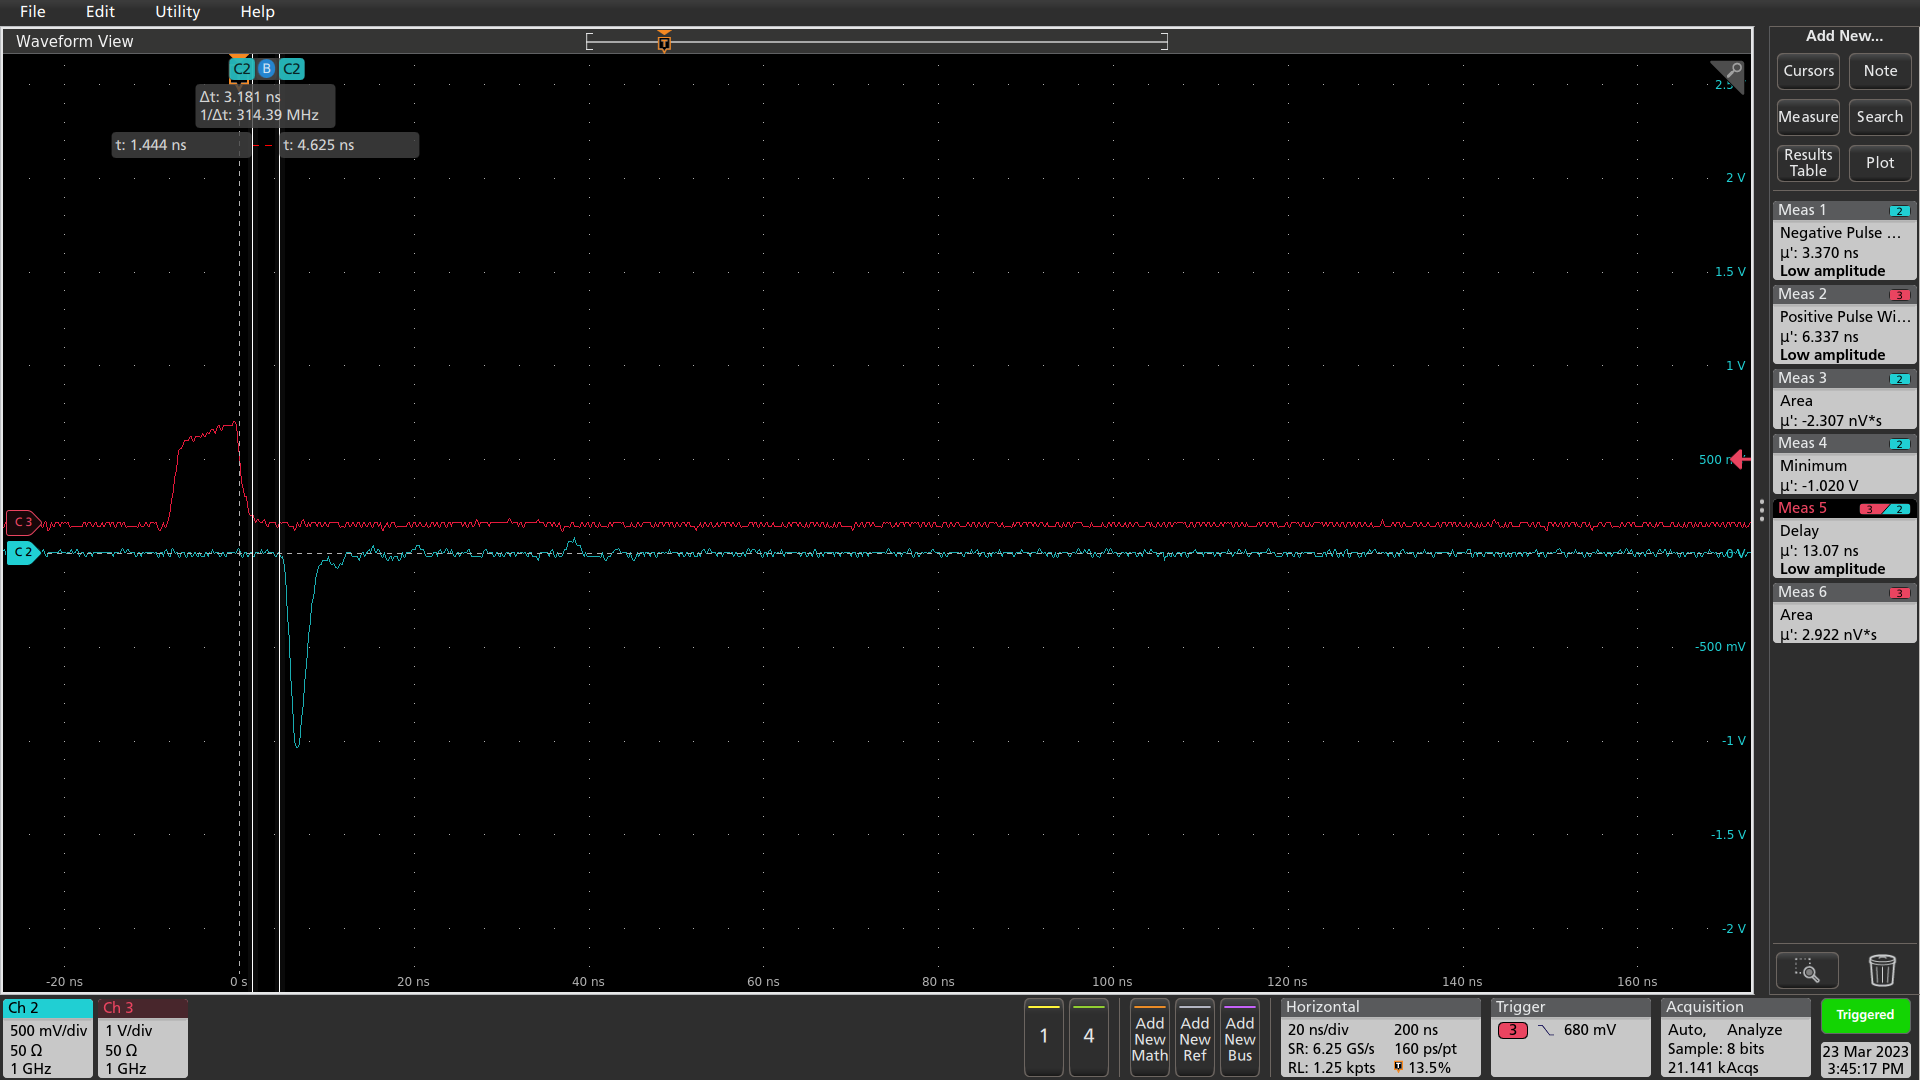
\includegraphics[scale=0.3]{800420nh47pf_000.png}
\caption{EPC8004 Pulse Shape\label{fig:EPC8004PulseShape}}
\end{figure}

\begin{figure}[htbp]
\centering
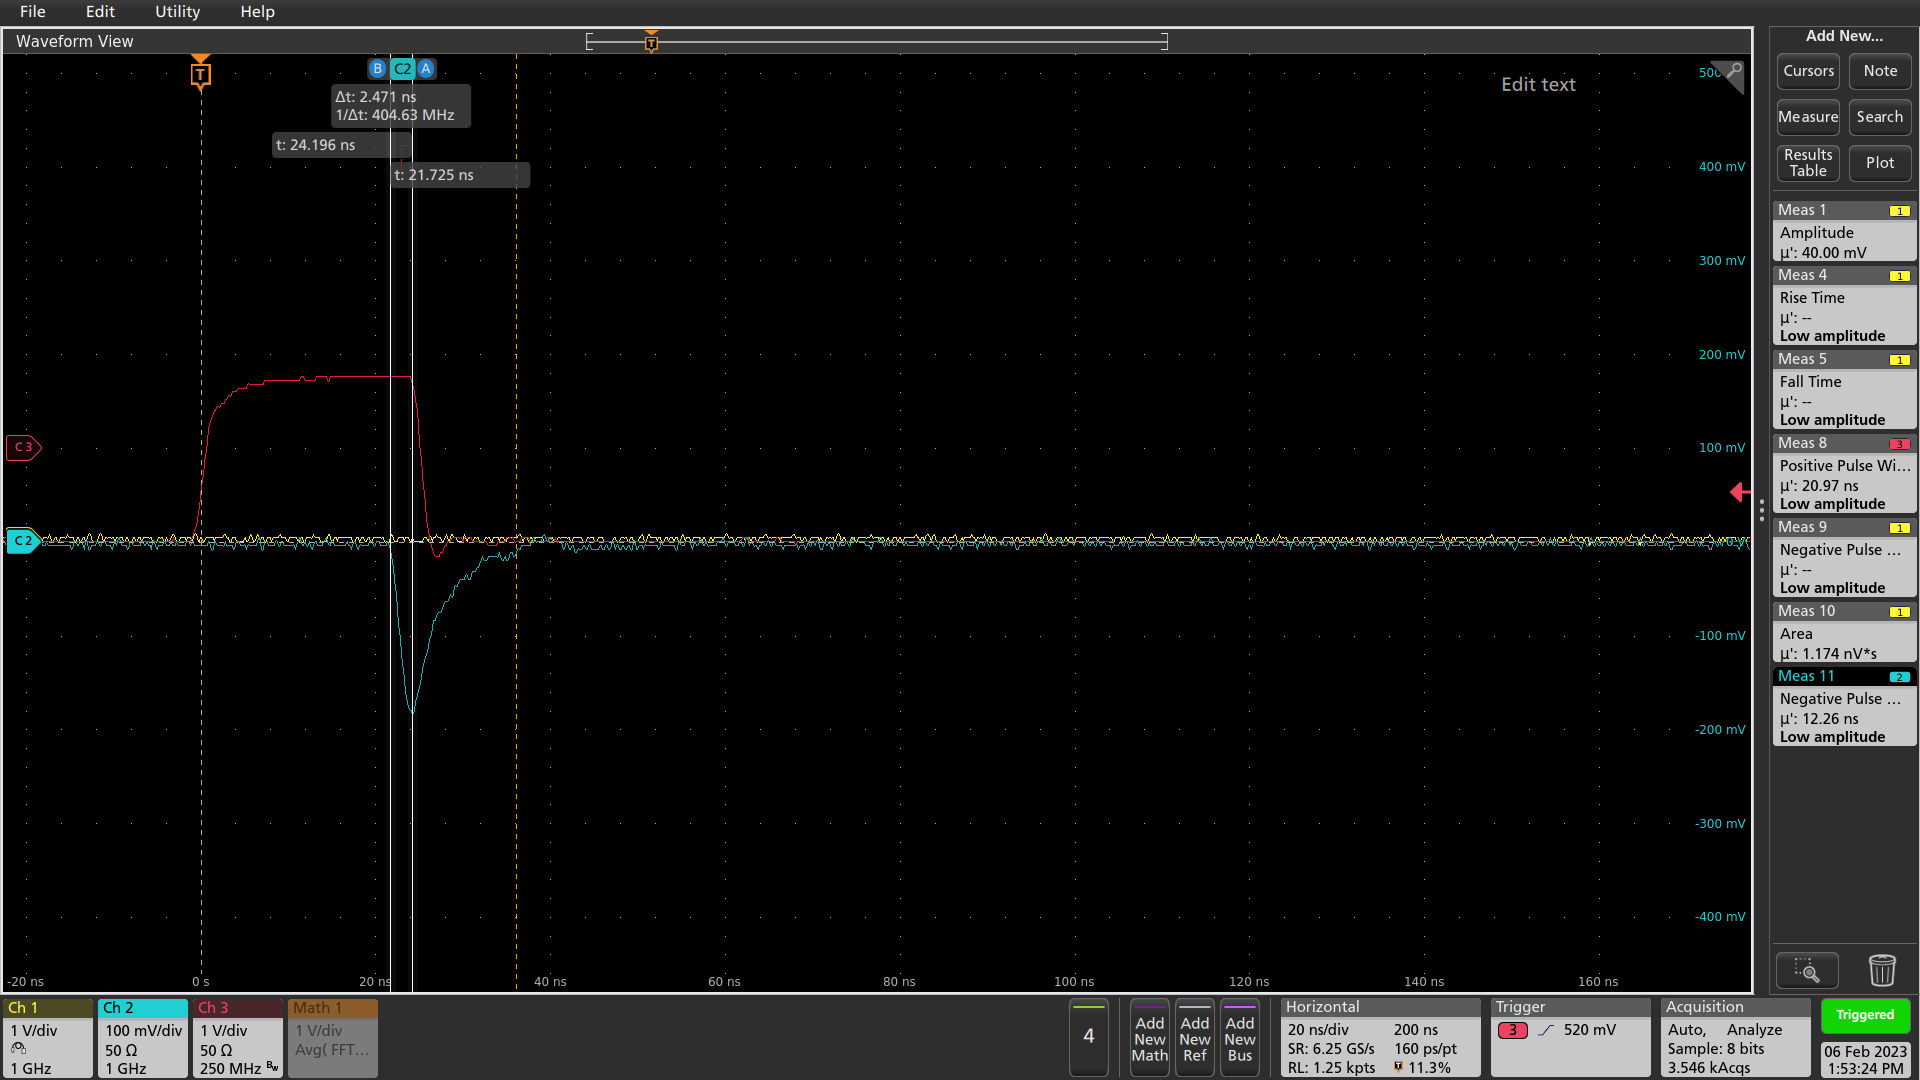
\includegraphics[scale=0.3]{RCTHTest1 no inductor.png}
\caption{Pulsing Circuit With No Inductor and Resistor\label{fig:NoRLPulse}}
\end{figure}

\begin{figure}[htbp]
\centering
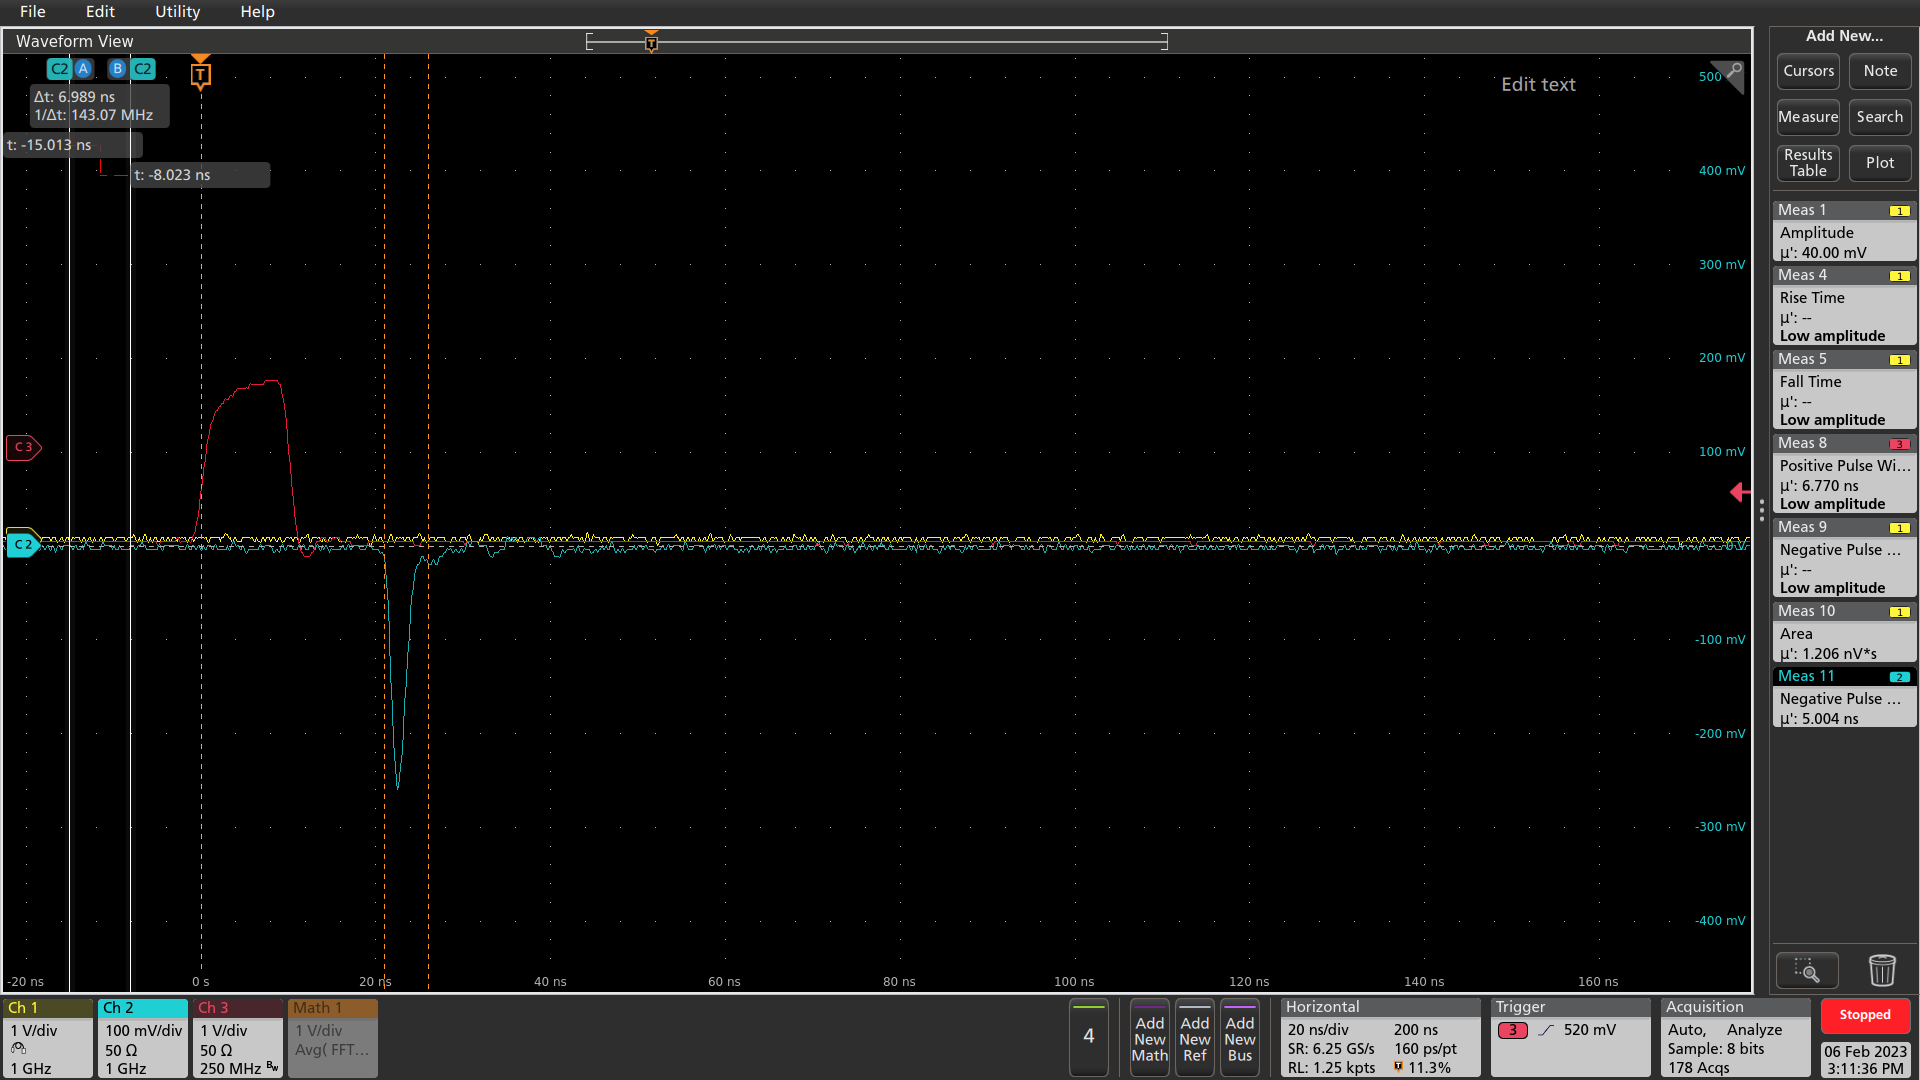
\includegraphics[scale=0.3]{RCTHTest1 inductor circuit.png}
\caption{Pulsing Circuit With Inductor and Resistor\label{fig:RLPulse}}
\end{figure}

%Check for diikey LED, that will will be in the future and check for LED part numbers
\subsubsection{Testing}

For testing purposes, the previous-generation United Kingdom Light Injection (UKLI) motherboard and associated software were utilised in conjunction with a prototype of the next-generation pulser board. This prototype consisted of four distinct circuit variants: one employing the EPC8004 switch, another utilising the EPC2012 switch, a third using the same high-speed transistor, BFR92, as implemented in the legacy system, and a fourth variant incorporating an EPC2012 gate in a through-hole package instead of the standard 0805 surface-mount footprint. We also done further evaluation using our latest pulser board prototype once we had them on hand.
Following comparative performance evaluations, the configuration using the EPC8004 switch was selected for continued use. While both the EPC8004 and EPC2012 switches exhibited similar electrical characteristics, the EPC8004 offered superior performance due to its lower parasitic capacitance, without any additional cost.
The OCS assembly was housed within a dark box during testing, and a 3D-printed fibre coupler was employed to facilitate light delivery. The initial focus of the evaluation was on the shape of the generated optical pulse.
During component selection, it was observed that the LED previously sourced from Mouser (ATS2012UV385 by Kingbright) provided acceptable performance in terms of electrical characteristics, but the optical output was suboptimal. Additionally, this LED was found to be out of stock and obsolete at the time after testing, precluding further procurement.
Subsequently, four ultraviolet LEDs from LC LED were assessed—two emitting at 365,~nm and two at 395~nm—each in both 0805 and 0603 surface-mount packages. Results demonstrated that the 0805 package LEDs provided significantly better optical coupling efficiency with the FP400URT optical fibre. Furthermore, the 365~nm variant exhibited superior optical power output relative to the 395~nm counterparts.
Based on these findings, the LC LED UT-67UV365P~\cite{ut-67uv365p} 365~nm LED was selected as the most suitable LED for this application.



\subsection{LVDS to TTL Converter}

The DS90C402 \cite{DS90C402} from Texas Instruments was selected as the LVDS-to-TTL conversion solution. This device is a dual-channel converter, chosen primarily for its fast switching characteristics—offering both rise and fall times of approximately 500~ps. It operates at 5~V and provides 5~V TTL output levels, which aligns well with the requirements of the downstream switching circuitry. The inclusion of two channels is particularly advantageous, as it enables the generation of sub-nanosecond differential pulses by precisely offsetting the channels, as described in Switch Selection. Among commercially available devices with these specifications, the DS90C402 is the fastest and is readily available through multiple distributors.

The associated circuit was implemented in accordance with the manufacturer's recommendations provided in the datasheet. Decoupling capacitor was placed in close proximity to the power supply pin to minimise voltage ripple. Output traces were routed using polygon fills to reduce impedance and enhance signal integrity, and a continuous ground plane was placed beneath the signal layers to improve shielding and minimise electromagnetic interference.

\begin{figure}[htbp]
\centering
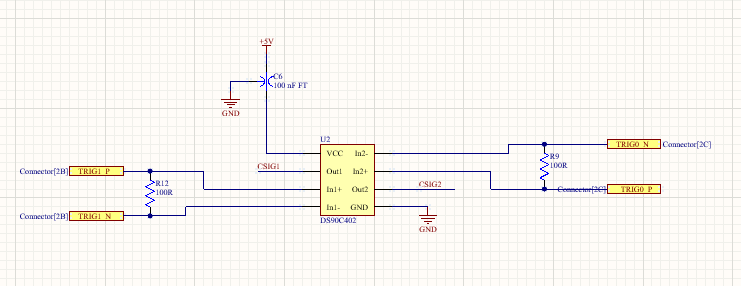
\includegraphics[scale=0.5]{LVDS-TTL Converter.png}
\caption{LVDS-TTL Converter Schematic\label{fig:i}}
\end{figure}


\subsection{Power supplies}

Each pulser board is required to incorporate a variable voltage power supply dedicated to driving the LED, with an adjustable output range from 3~V to 12~V. This supply is used exclusively to modulate the LED’s light output by varying the forward voltage, and consequently the current. The design specification also necessitates that the power supply be remotely controllable—i.e., capable of being switched on or off via a simple logic-level signal.

For this purpose, the LT1963A \cite{LT1963} adjustable low-dropout linear regulator was selected. This regulator has demonstrated reliable performance in previous pulser board iterations and offers a favourable balance of cost-effectiveness and controllability. The implementation includes standard filtering and decoupling, with layout details provided in Figure~\ref{fig:LT1963Layout}. The schematic provided~\ref{fig:12VVariablePSU} is an early version used for prototyping, the adjustable circuit has been simulated and will be tested shortly, and the Enable circuit has been tested, modified and simplified, updated schematics will be provided with V1.0 circuit.

\begin{figure}[htbp]
\centering
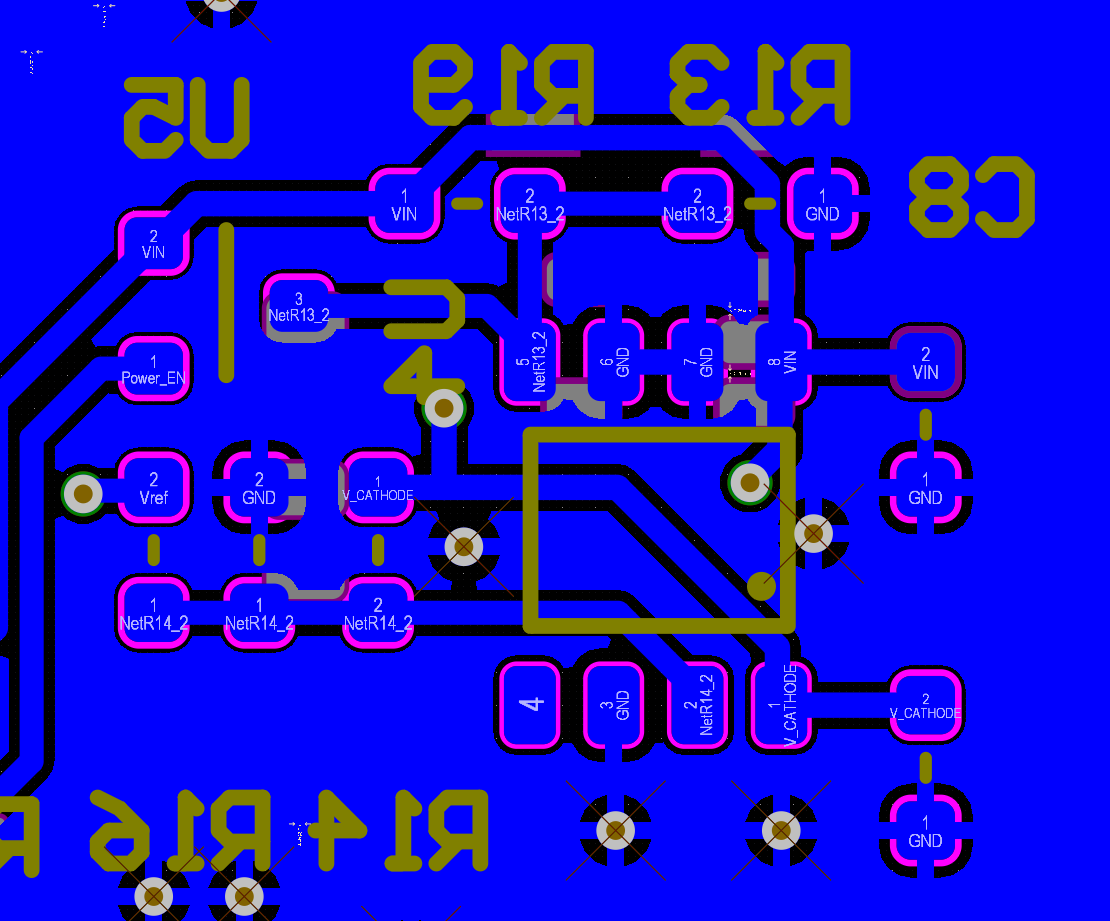
\includegraphics[scale=0.5]{LT1963layout.png}
\caption{LT1963 Layout\label{fig:LT1963Layout}}
\end{figure}

In addition to the variable LED supply, each board requires a stable 5~V supply to power both the DS90C402 LVDS-to-TTL converter and the LMG1020 gate driver. Unlike the LED supply, this rail remains continuously powered. The 5~V supply is provided by an LM2937-5 \cite{LM2347-5}, a fixed-output linear voltage regulator, which has been successfully employed in various high-speed and low-noise applications within the laboratory. The associated circuit schematic~\ref{fig:5VCircuit} and layout are shown in Figure~\ref{fig:LM29375Layout}.

\begin{figure}[htbp]
\centering
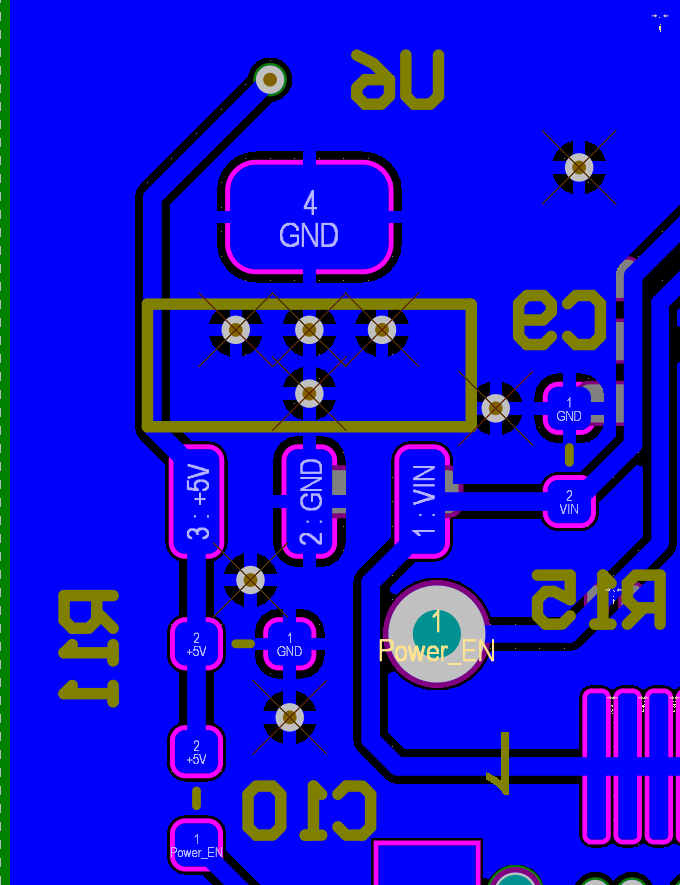
\includegraphics[scale=0.5]{LM29375Layout.png}
\caption{LM2937-5 Layout\label{fig:LM29375Layout}}
\end{figure}


To meet system-level design constraints, each pulser board is equipped with its own independent 12~V input supply, ensuring that LED output intensity can be individually controlled on a per-board basis. However, the 5~V supply is common across all boards and derived locally on each pulser module. This approach allows for localised filtering and minimal power distribution path lengths, reducing the risk of noise coupling and voltage drop considerations that are particularly critical in high-speed circuit applications.

Power is supplied to each board via the Eurocard backplane. The 12~V input from the Eurocard simultaneously feeds both the variable (LED) and fixed (logic) power regulators on the pulser board. The LED enable function is controlled via a 5~V logic signal originating from the Eurocard’s GPIO interface. Additionally, a DAC output from the Eurocard provides a voltage control signal to the adjustment pin of the LT1963A regulator on each pulser board, thereby allowing precise, programmable control of light intensity.

\begin{figure}[htbp]
\centering
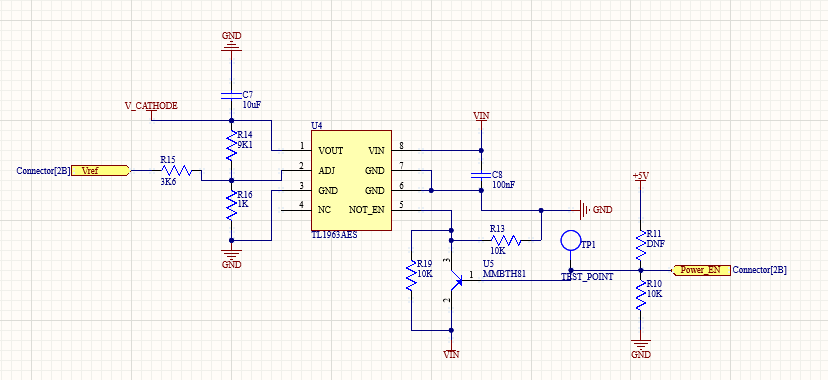
\includegraphics[scale=0.5]{12VVariablePSU.png}
\caption{12V Circuit Schematics\label{fig:12VVariablePSU}}
\end{figure}

\begin{figure}[htbp]
\centering
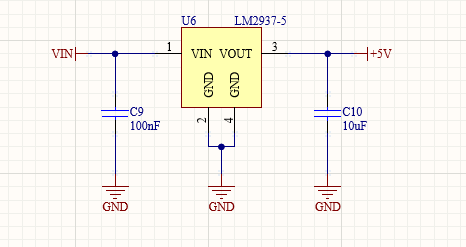
\includegraphics[scale=0.5]{5VCircuit.png}
\caption{5V circuit schematics\label{fig:5VCircuit}}
\end{figure}

\subsection{Connector}

The previous board connector was deemed bulky and expensive, which lead to the processof finding a more suitable alternative. Following an evaluation of commercially available options, the Phoenix Contact female connector 1331962 \cite{1331962} was selected.

This connector offers several advantageous specifications: it is rated for \SI{500}{\volt}, features a low contact resistance of \SI{40}{\milli\ohm}, supports a maximum current of \SI{0.5}{\ampere}, and is capable of signal transmission up to \SI{20}{\giga\bit\per\second}. In addition, it is cost-effective, priced at approximately \pounds 0.50 per unit.


Multiple height variants are available within the same series, facilitating flexible mechanical integration within the Eurocard crate system. The compact footprint of the connector allows for a reduced PCB form factor.

The selection of this connector was based on several key factors. Its wide availability ensures ease of procurement. The connector series offers multiple height options with identical pin counts, allowing for mechanical adaptability within the Eurocard crate system. It is economically advantageous, with both male and female variants priced at approximately \pounds 0.50 per unit. Electrically, the high-frequency performance supports reliable LVDS signal transmission. Additionally, the compact footprint of the connector is well-suited to space-constrained PCB layouts.

A figure illustrating the connector and corresponding circuit layout is provided below in Figure~\ref{fig:Connector}.

\begin{figure}[htbp]
\centering
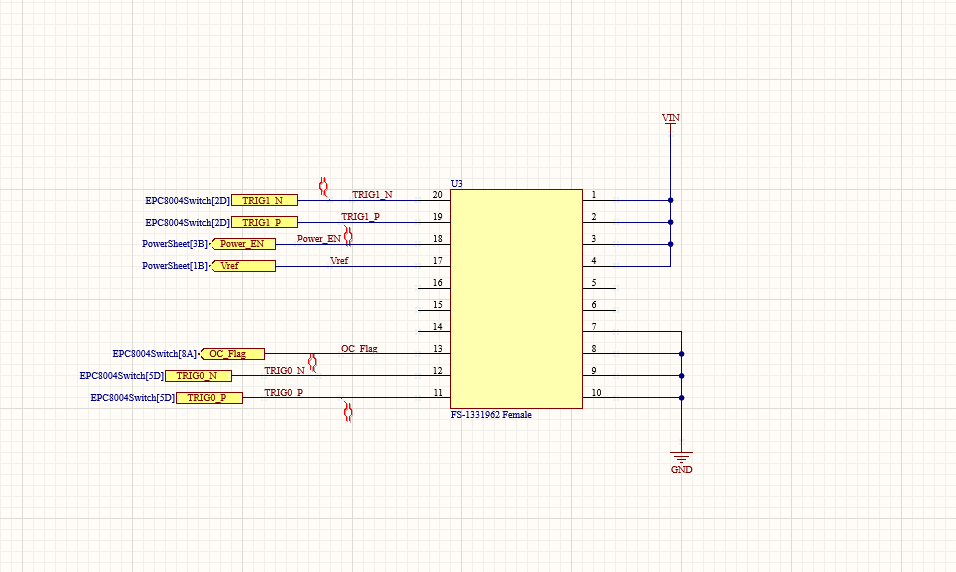
\includegraphics[scale=0.5]{Connector.png}
\caption{Connector Schematics\label{fig:Connector}}
\end{figure}


\subsection{Fibre Coupler}

During the prototyping phase, improvements were made to the PCB layout to better accommodate a fibre coupler. As a result, the current design includes provisions for precise mechanical mounting and alignment. Specifically, two mounting holes for M2 screws have been incorporated, enabling the 3D-printed coupler to be firmly secured to the board (see Figure~\ref{fig:OldFibreCouplerDesign}). In addition, two dowel holes have been added to guide the coupler into position, ensuring accurate alignment over the LED. Given the tolerances associated with PCB fabrication and 3D printing, an alignment accuracy of approximately \SI{100}{\micro\metre} is expected.

\begin{figure}[htbp]
\centering
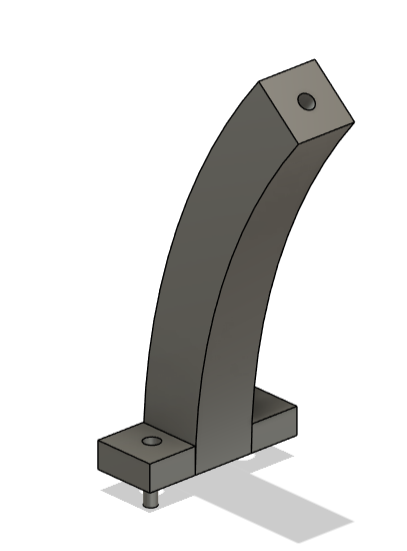
\includegraphics[scale=0.5]{OldFibreCouplerDesign.png}
\caption{Old Fibre Coupler Design\label{fig:OldFibreCouplerDesign}}
\end{figure}

To optimise the electrical path, capacitors have been repositioned as close as possible to the LEDs. This minimises parasitic inductance and resistance, while enabling a centralised layout of larger components. The resulting configuration creates a compact chamber housing both the LEDs and associated capacitors.

An earlier design for the fibre coupler, which assumed uniform fibre lengths for all channels, has since been abandoned. A revised approach adopts five different fibre lengths, necessitating individual light attenuation for each channel. This attenuation will be implemented within the coupler itself, allowing the LED output to remain within the electronically controlled dynamic range.

The proposed design is modular, consisting of three components: a base section mounted to the pulser PCB, a top section into which the fibres will be epoxied, and an intermediate attenuator element. The latter will serve to space the fibre from the LED and thereby adjust the optical coupling efficiency to achieve the required attenuation.

While an initial prototype will be developed for functional testing, the full design and validation of the fibre coupler will be undertaken as part of an undergraduate project during the 2025/26 academic year, under my supervision. Should the project timeline require faster iteration, personal prototyping will also be pursued.

The fibre coupler will be fabricated via stereolithography (SLA) using a black resin to minimise light transmission through the material. Additional light-tight testing will be conducted, and black paint may be applied if further sealing is required. Furthermore, laser-cut rubber gaskets will be introduced at interface points to ensure optimal optical isolation and mechanical sealing.

\subsection{Production}

We will use PCB Train, they are local and reasonably priced, they are proved to produce boards in good quality. Estimated BOM cost is £12.27 per board, which is £1,496.94 for 122 units or £1,840.5 for 150 unit, and production is £4073.48 for 122 units for 15 days lead time, or £3985 for 150 units at 25 days lead time~\ref{fig:PCBTrainOrder}

\begin{figure}[htbp]
\centering
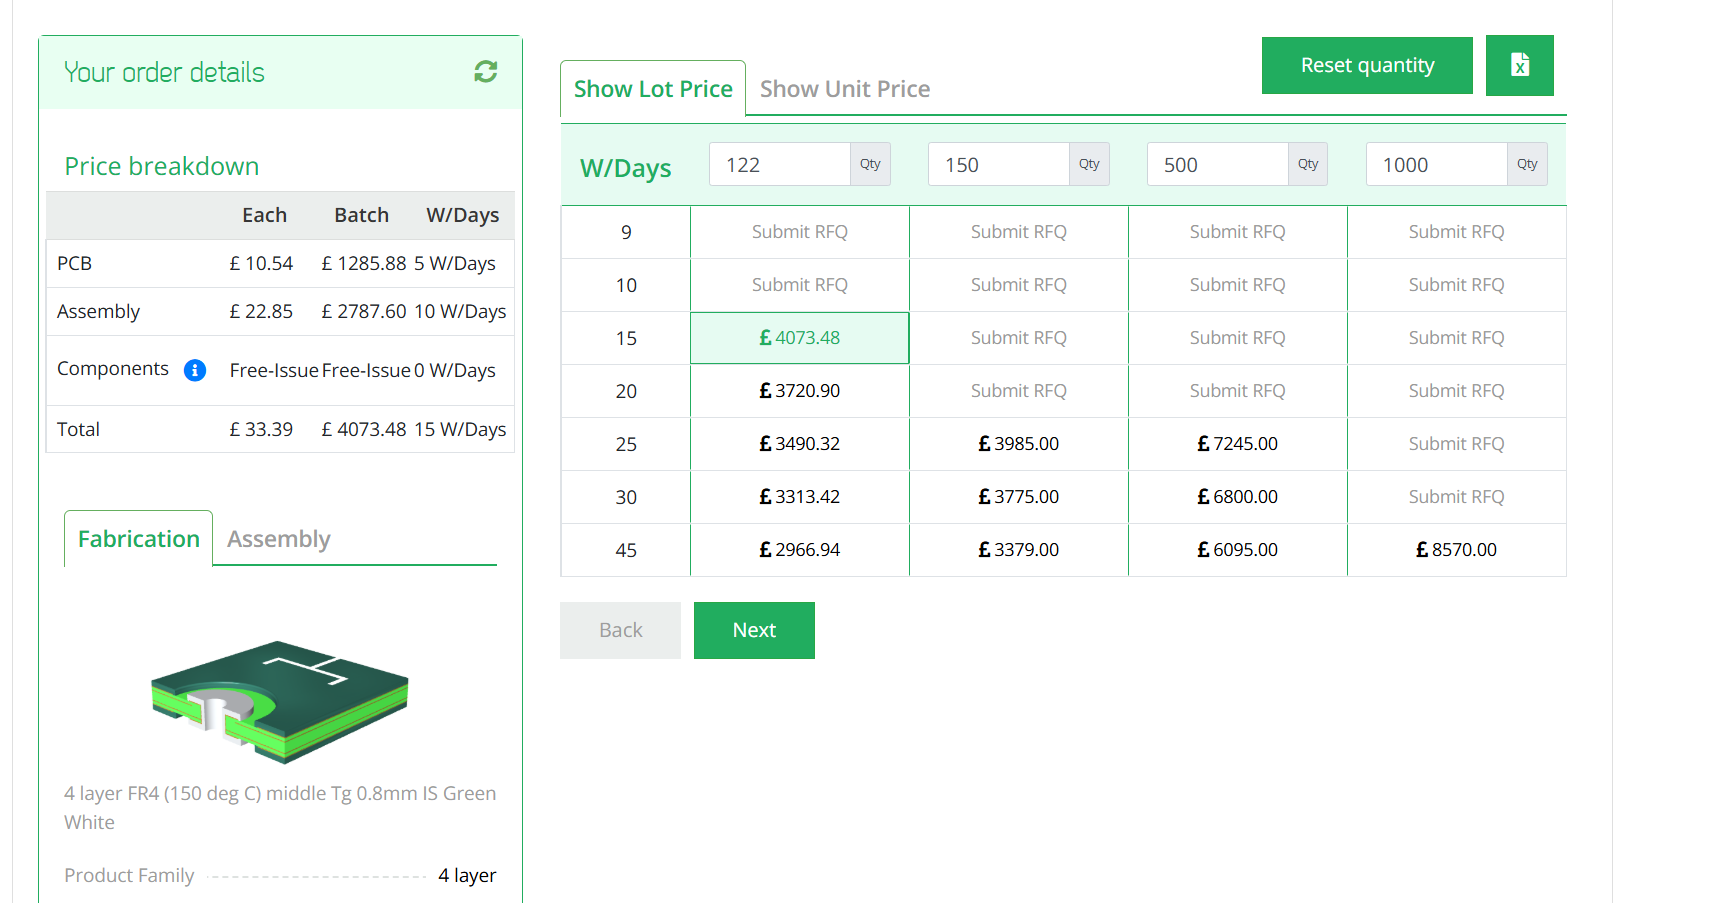
\includegraphics[scale=0.5]{PCBTrainOrder.png}
\caption{PCBTrain PCB production and assembly costs\label{fig:PCBTrainOrder}}
\end{figure}


\subsection{Changes expected from V0.9 to V1,0}

\subsubsection{LED and switching circuit}

There will be minimal changes for the LED and switching circuit. The changes will be made to the position of the switching devices, just placing them a bit closer to each other to reduce transmission line length. The LED will highly likely stay the LC LED UT-67UV365P 365nm 0805 LED, but further LED tests will be done, as it takes short time, and we might find LEDs in the future which will be easy to replace due to standardised footprints.

\subsubsection{LVDS-to-TTL converter}

No Changes expected for this circuit

\subsubsection{Power supplies}

Reverse voltage bias will be removed as I found do change between normal and reverse bias as per photon output. The overcurrent protection and power enable circuit will be reworked.

\subsubsection{Connector}

No changes

\subsubsection{Fibre coupler}

A brand new fibre coupler will be designed due to the recent requirement changes regarding the different fibre lengths.



\section{Server Rack and Cooling}

There will be two 42U server racks with 800mm depth. The front of the server rack will be used for electrical connections and displays, and the reverse/internal will be used only for fibre routing. The server racks will inlcude Uninterruptible Power Supplies (UPS) for safe power delivery and for power processing, as we are not sure how stable the power is going to be at all times. Each rack will include an air conditioning unit as well, to have a controlled temperature and to remove humidity from the air, as it will be around 100 per cent air humidity. We are not sure how this humidity would effect the LED Light Injection System, but we know that the optical switches for the laser calibration system requires lower humidity levels, so we just air condition both server racks to remove this variable. All of these are widely available and will be chosen closer to installation.

\section{LED Monitoring}

We are going to use PMTs to monitor the LEDs in a very similar way as it works in Super-Kamiokande. This is the most accurate and cost effective way of doing it. We are expected to use Hamamatsu H10721-210 PMTs and due to the 8mm diameter window area we can attach up to 16 LEDs, which mean each crate will use 2 PMTs. Each PMT will be powered by a unique low cost power supply that is being used in SK, but instead in a large enclosure it will be inside a small 2-3 U server rack. The signals from the PMTs then will go to the dedicated HK electronics channels that are set up for for monitoring.

\section{Control System for LEDs}

The LEDs are driven by a differential LVDS signal originating from the FPGA. The FPGA in use is the Genesys 2 \cite{Genesys2} development board, which operates a pulsing VHDL module clocked at \SI{300}{\mega\hertz}. Pulses are generated on the rising edge of this clock, and toggling the output (i.e., asserting and then deasserting the trigger) requires a minimum of two clock cycles. Consequently, the shortest achievable pulse duration in this configuration is \SI{3.3}{\nano\second}.

One of the main limitations of this setup is the coarse time resolution: pulse durations are effectively constrained to integer multiples of \SI{3.3}{\nano\second}. To achieve a broader and more finely resolved spectrum of optical injection into the detector, improved temporal precision is necessary. This is accomplished using the Xilinx \texttt{IODELAY} primitive, originally designed for high-speed interface timing alignment. The \texttt{IODELAY} module permits fine-tuning of signal timing to account for PCB trace mismatches, and in this application, it is repurposed to introduce controlled delays between pulses.

To generate shorter pulses, two identical signals are created, one of which is delayed using \texttt{IODELAY}. These signals are then combined using a logical \texttt{AND} operation, producing a narrower pulse. Since the \texttt{IODELAY} module requires one clock cycle to process the input, both signals—regardless of whether they are delayed—must pass through an \texttt{IODELAY} stage to ensure temporal synchronisation.

Conversely, to produce longer pulses, the same methodology is applied, but the signals are combined using a logical \texttt{OR} gate instead. This approach extends the pulse width beyond the base clock resolution, enabling pulse durations ranging from approximately \SI{1.5}{\nano\second} to \SI{4.5}{\nano\second} in 49 discrete steps. The lower bound is determined by the threshold of the LVDS-to-TTL converter, which does not respond to pulses shorter than approximately \SI{1.5}{\nano\second} .

For channels using the longest optical fibres, this extended range is sufficient, given the intrinsic dispersion of around \SI{5}{\nano\second}. However, shorter fibres require additional pulse shaping. To this end, an additional mechanism is implemented using a \texttt{for} loop structure within the FPGA logic. This allows the pulse to persist for multiple clock cycles, effectively producing longer pulses by repetition. However, due to FPGA architecture constraints, each iteration of the loop consumes a clock cycle, necessitating careful timing control. For instance, to produce a \SI{6.6}{\nano\second} pulse, the loop must be configured for two cycles, accounting for the loop overhead.

Further refinement is under investigation through the daisy-chaining of multiple \texttt{IODELAY} modules. This would enable sub-nanosecond granularity by introducing additional intermediate delay steps. While promising, this technique requires further validation and testing.

The pulse control data structure is currently under development. There are 2 types of pulse description is considered. First option, the software interface would require two parameters per channel: a \textit{coarse} step and a \textit{fine} step, reflecting the approach used in the SK system. The other option would be just a single variable and then simple logic turning that variable into the \textit{coarse} and \textit{fine} step that the internal logic requires, Two hardware modules are planned: one for generating the single shortest possible pulse (to minimise latency), and another for multi-cycle pulses using programmable duration. A selection logic will assess the input and route it to the appropriate module based on the desired pulse characteristics.

Each LED channel will be controlled independently, allowing for unique pulse configurations across channels. The global trigger will be derived from the system clock, and each channel will pulse in a predefined sequence while triggered from the global trigger. This architecture also supports simultaneous pulsing of multiple channels. Should asynchronous behaviour be required, additional per-channel delay logic can be implemented.

Given the five distinct fibre lengths used in the system, each channel group will also include a configurable delay offset to compensate for propagation time differences. These group delays will be calibrated and fixed, with the option of fine-tuning individual channels post-deployment if necessary.

The FPGA programming remains in active development. Inter-crate communication protocols and synchronisation are currently under integration and testing.

\section{Crate Electronics}

\subsection{Overview}

The system specification calls for control of up to 122 LED channels, significantly exceeding the channel counts used in current systems such as Super-Kamiokande or LUX-ZEPLIN. To manage this complexity, the design prioritises ease of use, maintainability, and straightforward deployment, particularly given that the server racks will accommodate hundreds of optical fibres.

To achieve this, a system concept originally developed by our ATLAS collaborators, specifically by Ashley Greenal, has been adapted. The original design utilises a Genesys 2 FPGA integrated into a half-width Verotec KM6-2 \cite{KM6-2} Eurocard-compatible crate for testing purposes. This concept has been extended to a full 19-inch rack width, enabling the integration of up to 36 pulser boards within a single crate.

Each FPGA is capable of interfacing with up to 38 pulser boards, thereby maximising the utilisation of available LVDS differential pairs, with an additional pair reserved for the laser trigger signal. This configuration ensures full use of the Genesys 2’s I/O capacity while maintaining flexibility for future expansion.

The system architecture consists of three primary components:

\begin{itemize}
\item \textbf{Blade}: Interfaces directly with the FPGA via the FMC connector, distributing all differential signals into the crate system.
\item \textbf{Backplane}: Routes differential signals to the pulser boards and provides the primary power distribution, accepting \SI{12}{\volt} and \SI{\pm5}{\volt} inputs.
\item \textbf{Eurocards}: Host the pulser boards, receive power and differential signals from the backplane, and incorporate the necessary circuitry for laser triggering.
\end{itemize}

This modular approach ensures scalability and facilitates debugging, replacement, and upgrades. It also provides a robust foundation for managing high channel counts while maintaining signal integrity and synchronisation across the system.

\subsection{Blade}

The Blade is a simple, 8 layer board, that has a SEAM-40-06.5-L-10-2-A-K-TR \cite{SamtecSeam} connector which is a direct fit for the Genesys 2's FMC connector and it has a PCIE 16X connector at the edge for connectivity to the Backplane. The PCIE was selected by Ashley Greenal as it is a well documented standard connector and there are a great amount of connectors out that that can be bought easily. While we are using PCIE connectors we are not using PCIE standards for communication. This is a very densee PCB with all the differential tracks on it so burried vias and multiple layers will be used. See Figure~\ref{fig:BladeWIP} for a work in progress version.

\begin{figure}[htbp]
\centering
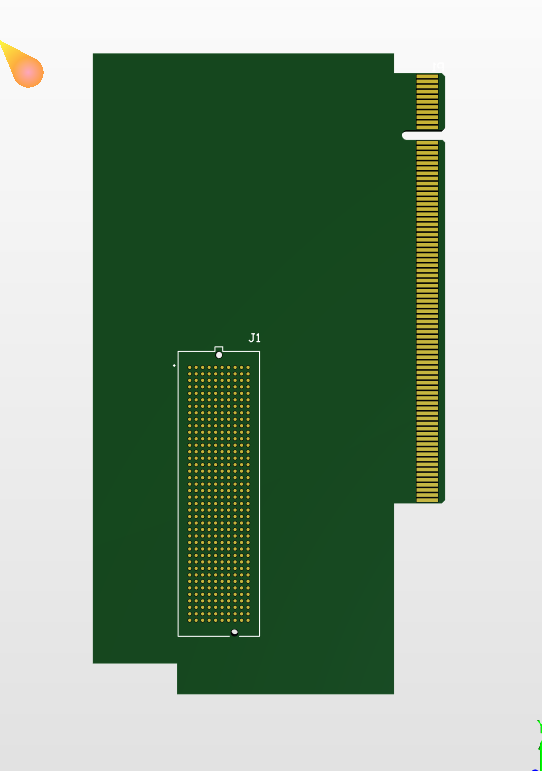
\includegraphics[scale=0.5]{G2BladeWIP.png}
\caption{Blade Work in Progress\label{fig:BladeWIP}}
\end{figure}

\subsection{Backplane}

The Backplane serves two primary functions: the distribution of differential signals from the Blade to the Eurocards, and the reception and distribution of power throughout the crate system. It accepts external power inputs of \SI{12}{\volt} and \SI{\pm5}{\volt}, and includes a basic regulation circuit to stabilise these supply voltages for downstream use.

Given the mechanical constraints and routing complexity, the Backplane is implemented as a four-layer PCB with impedance-controlled traces to ensure signal integrity across all differential pairs. It features a single PCIe x16 connector to interface with the Blade, and three PCIe x8 connectors to interface with the Eurocards.

The Eurocards are positioned at slots 2, 8, and 64 within the crate. This arrangement creates two symmetrical chambers with  48 units spacing between cards, ensuring adequate space to accommodate the minimum long-term bend radius of the FP400URT optical fibres. This layout balances mechanical reliability with signal routing efficiency and supports long-term maintainability of the system. See Figure~\ref{fig:BackplaneWIP} for a work in progress version.

\begin{figure}[htbp]
\centering
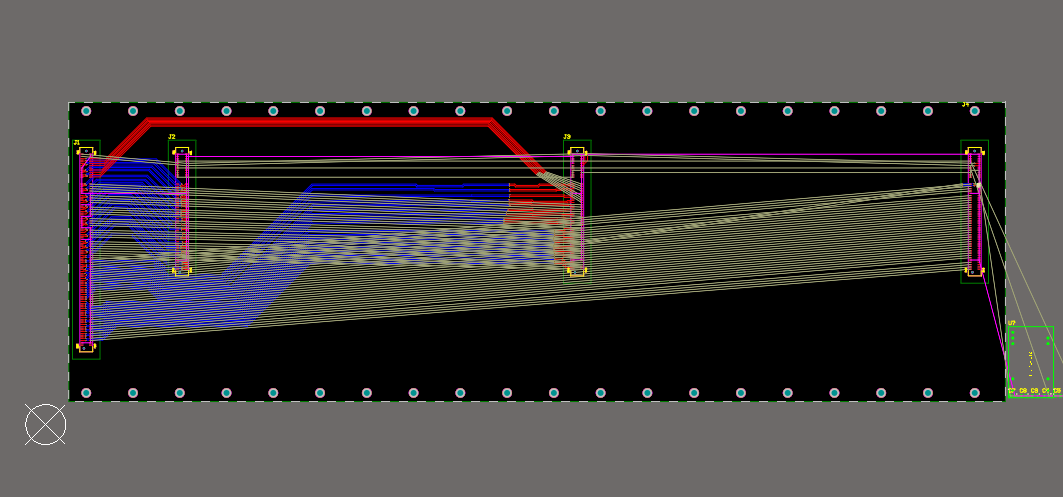
\includegraphics[scale=0.5]{BackplaneWIP.png}
\caption{Backplane Work in Progress\label{fig:BackplaneWIP}}
\end{figure}

\subsection{Eurocard}

The Eurocard format defines the physical and electrical standard for the crate system, hence the naming convention. Each Eurocard is equipped with a PCIe x8 connector for interfacing with the Backplane and is designed to host up to 18 pulser boards—nine mounted on each face. Pulser boards connect via FS-1332120 Male\cite{1332120} connectors, and each socket includes two mounting holes for mechanical standoffs.

The board layout on each side consists of two staggered rows: five sockets in the back row and four in the front. The two faces are laterally offset by approximately \SI{10}{\milli\metre} to prevent interference or fibre clashes when the system is fully populated and enclosed within the crate chamber. This offset ensures smooth fibre routing and accommodates the bend radius requirements of FP400URT fibres.

Power distribution within each Eurocard is handled by a THD 12-1212 \cite{THD121212}\SI{12}{\volt} DC-DC regulator. This regulator provides local power isolation for the pulser boards and includes a control pin connected to a PCA9698 \cite{PCA9698} 40-pin GPIO expander. This allows for system-level control, enabling or disabling all pulser boards on a card—an essential feature during power-up, especially when the FPGA may inadvertently drive all differential outputs high during reprogramming.

The GPIO expander is responsible for enabling the local \SI{12}{\volt} regulator and for selectively powering individual pulser boards. This facilitates fault isolation and power savings in channels that are inactive or disconnected. Additional GPIO pins are assigned to monitor output voltage levels via the overcurrent sensing circuitry.

To provide per-channel LED power control, an AD5673 \cite{AD5673} DAC is included. It outputs analogue control voltages to the onboard adjustable regulators on each pulser board, allowing for independent LED drive voltage per channel. Both the GPIO and DAC devices communicate with the system over the I\textsuperscript{2}C protocol.

For laser synchronisation, the Eurocard includes a differential-to-NIM conversion stage. This consists of an LVDS-to-TTL converter identical to that used on the pulser boards, followed by a TTL-to-NIM converter. This ensures compatibility with legacy NIM-based timing systems used in external laser triggering. See Figure~\ref{fig:EurocardWIP} for a work in progress version.

\begin{figure}[htbp]
\centering
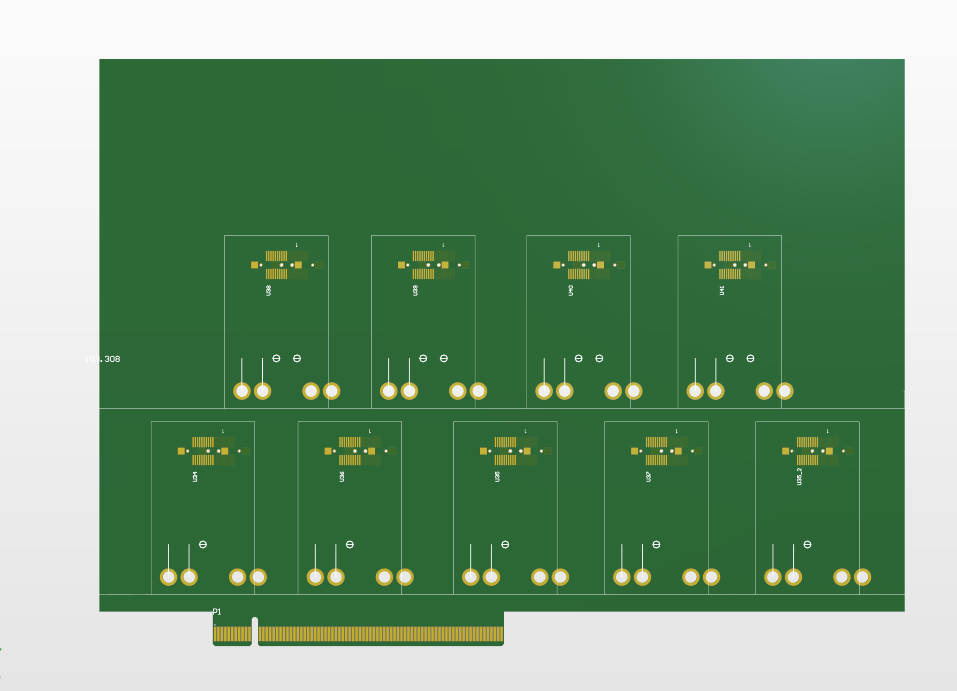
\includegraphics[scale=0.5]{EurocardWIP.png}
\caption{Eurocard Work in Progress\label{fig:EurocardWIP}}
\end{figure}










\appendix










% Bibliography

%% [A] Recommended: using JHEP.bst file
%% \bibliographystyle{JHEP}
%% \bibliography{biblio.bib}

%% or
%% [B] Manual formatting (see below)
%% (i) We suggest to always provide author, title and journal data or doi:
%% in short all the informations that clearly identify a document.
%% (ii) please avoid comments such as "For a review'', "For some examples",
%% "and references therein" or move them in the text. In general, please leave only references in the bibliography and move all
%% accessory text in footnotes.
%% (iii) Also, please have only one work for each \bibitem.

\printbibliography

\end{document}
